\section{Results}
This section contains results of the planning framework and is subdivided into three subsections: uncontested results, contested results, and multi-rate comparisons.  
\subsection{\label{sec:setup} Baseline and Setup}
The experiments in this section compare the results of the framework given in equation (\ref{eqn:finalObjective}) with a baseline that models the general behavior of bus drivers at the Utah Transit Authority (UTA) in SLC, Utah and the planning framework from \cite{He_2022_Battery}. All methods use a MILP to find an optimal solution and are solved up to a 2\% gap using Gurobi \cite{gurobi}.
\par According to UTA, bus drivers generally charge whenever possible. Our baseline scenario reflects this default bus driver behavior using an objective function that maximizes the number of charging instances, which is computed as the sum of group flow values, resulting in the objective function
\begin{equation}
	\underset{\mathbf{y}}{\text{max}} \ \mathbf{1}^TB\mathbf{y},
\end{equation}
\par All other constraints are the same, which results in the baseline formulation 
\begin{equation}\label{eqn:finalBaselineObjective}
	\begin{matrix*}[c]
		\underset{\mathbf{y}}{\scalebox{1}{\text{max}}} \ \mathbf{1}^TB\mathbf{y} \ \text{subject to}\\
		\begin{bmatrix*}[l]
				\tilde{A} \\
				D_{\text{eq}} \\
				P
				\end{bmatrix*} \mathbf{y} = \begin{bmatrix*}[l]\mathbf{c}_f \\ \mathbf{d}_{\text{eq}}\\\mathbf{p} \end{bmatrix*}, \ \begin{bmatrix*}[l]
			\tilde{B} \\
			D_{\text{ineq}} \\ 
			P_{\text{max}} \\
			P_{\text{on}} \\
			P_{\text{off}}
			\end{bmatrix*}\mathbf{y} \le \begin{bmatrix*}\mathbf{1} \\ \mathbf{d}_{\text{ineq}} \\ \mathbf{0} \\ \mathbf{0} \\ \mathbf{0} \end{bmatrix*}
	\end{matrix*}.
\end{equation}
\par Each experiment is run using a five minute timestep such that the time difference between $t_k$ and $t_{k+1}$ is five minutes.  Four charge rates are used during the following experiments: $\bar{a}_1 = 0.9851$, $\bar{a}_2 = 0.9418$, $\bar{a}_3 = 0.9003$, and $\bar{a}_4 = 0.8607$.  Each value for $\bar{a}$ represents a different charge rate and is referenced by how much time it would take a bus to charge from $0$\% to $99$\%. For the rates used in the following set of experiments, a bus would need 25.58 hours to charge from 0\% to 99\% with $\bar{a}_1$, 6.4 hours with $\bar{a}_2$, 3.65 with $\bar{a}_3$, and 2.56 with $\bar{a}_4$. 
\par Night charging uses a single charge rate of $\bar{a}_1$ for all experiments. Experiments with single rate day charging use $\bar{a}_4$, and multi-rate experiments incorporate four charge options: $\bar{a}_1$, $\bar{a}_2$, $\bar{a}_3$, and $\bar{a}_4$.
\par Uncontrolled loads are modeled with data from the TRAX Power Substation (TPSS) at the UTA Intermodel Hub site in Salt Lake City. It is also assumed that each bus starts and ends each day with an SOC of $80\%$ and has a maximum charge capacity of $100$ kWh.
\subsection{Uncontested Results}
This section explores performance in a scenario where there is one charger per bus during the day, making charge resources \textit{uncontested}. The optimal charge schedule associated with equation \ref{eqn:finalObjective} is compared with the schedule developed by the baseline in equation (\ref{eqn:finalBaselineObjective}). The total monthly cost is computed using the rates given in Rocky Mountain Power Schedule 8 and is computed in equation (\ref{eqn:RMPSchedule8}).
	\begin{equation}\label{eqn:RMPSchedule8}
		\begin{aligned}
			\text{cost} = & \text{ facilitiesPower}\cdot 4.81 + \text{onPeakPower}\cdot 15.73 + \\ 
			& \text{onPeakEnergy}\cdot 0.058282 + \text{offPeakEnergy}\cdot 0.029624
		\end{aligned}
	\end{equation}
	There is also a customer service charge of $71.00$ in the rate schedule, but because the service charge does not depend on a customer's behavior, it is ignored.
\par Because equation (\ref{eqn:RMPSchedule8}) is driven by facilities power, on-peak power, on-peak energy, and off-peak energy, these four criteria are used to evaluate the optimal and baseline charge plans.  Furthermore, because the on and off-peak energy charges contribute little to the cost differences, they have been grouped together for comparison.
\begin{figure}
	\centering
	\makeComparisonBarChartThree{media/costComparison5Bus5Chargers.csv}{Cost (Dollars)}{Baseline}{He et al.}{Optimized}
	\caption{Cost comparison between optimized and baseline algorithms.}
	\label{fig:costComparison}
\end{figure}
	\par  Fig.~\ref{fig:costComparison} compares the cost of energy, on-peak power, and facilities power for the baseline, \cite{He_2022_Battery}, and this work's scheduling strategies. Note how the schedule given by Hu et al. is similar in both energy costs and on-peak power charges but is more expensive in the facilities charge. These differences are expected as Hu et al. minimises cost of energy by charging during off-peak periods. Because there is minimal charging during on-peak times, the on-peak power charges reflect the uncontrolled loads and are therefore the same. The differences in facilities is present because He et al. does not include the overall maximum average power in their framework. 
	\par Additionally, the facilities and on-peak power costs for the baseline schedule are significantly larger than the optimized schedule.  To better understand the cost disparity, we observe the load profiles to identify how the optimized schedule avoids the costs incurred by the baseline.
\par Fig.~\ref{fig:totalPower1} shows the 15 minute average power for both the baseline and optimal schedules. Note how the optimal schedule incurs a lower average power for both on and off peak time intervals. The reduction in average power is what lead to the cost disparity between the on-peak and facilities power costs in Fig.~\ref{fig:costComparison}. 
\par The underlying behavior can be observed in Fig.~\ref{fig:powerPlot1}, which separates the loads into their controlled and uncontrolled constituents. Because the uncontrolled loads are shared between both scenarios, Fig.~\ref{fig:powerPlot1} shows the 15 minute average power for uncontrolled, optimal charging, and baseline charging loads. 
\par Observe how the optimized schedule avoids charging during on-peak hours and regulates each charge event to spread the power draw over larger periods of time. Furthermore, bus charging is avoided when uncontrolled loads are high, resulting in a reduced 15 minute average power.  Reducing the average power and not charging during on-peak periods results in the dramatic cost reduction shown in Fig. \ref{fig:costComparison}.

\begin{figure*}
	\centering
	\makeComparisonTotalPower{media/baseline5Bus5ChargerTotalPowerPlot.csv}{media/optimized5Bus5ChargerTotalPowerPlot.csv}{15-Minute Average Power (kW)}{Baseline}{Optimized}
	\caption{15-Minute average power for one day.}
	\label{fig:totalPower1}
\end{figure*} 
\begin{figure*}
	\centering
	\makeComparisonPower{media/baseline5Bus5ChargerPowerPlot.csv}{media/optimized5Bus5ChargerPowerPlot.csv}{15-Minute Average Power (kW)}{Baseline}{Optimized}
	\caption{Comparison between uncontrolled and bus loads.}
	\label{fig:powerPlot1}
\end{figure*}

\subsection{Contested Results}
This section observes the performance of the optimal schedule as charge resources become scarce, creating a contested environment. Resource contention is most prevalent when chargers are scarce and pushes buses to charge in non-ideal circumstances.  For example, if charging resources are saturated during off-peak hours, other buses might be forced to charge in the on-peak window. The impact of contention is measured as the change in monthly cost when the number of chargers is held constant and the number of buses increases. 
\par In this analysis, one charger is used and the number of buses is varied from five to eleven. Fig.~\ref{fig:contention1} shows the monthly cost as a function of the number of buses. Note the minimal cost increase per bus, where each successive bus costs around \$$75.00$, which approaches the cost of energy that is required to provide transit services.  Because the additional cost per bus is roughly the cost of energy, there are no additional facilities and on-peak power charges, showing that optimal charge plans also minimize cost in the presence of contention.
\begin{figure}
	\begin{tikzpicture}
		\begin{axis}[SmallPointPlot, xlabel=Number of Buses, ylabel=Total Monthly Cost, ymin=3000, xmax=11]
			\addplot[blue, only marks, mark size=3pt] coordinates {(5,3034.35) (6,3108.23) (7,3174.54) (8,3255.87) (9,3313.43) (10, 3391.16) (11, 3463.42)}; 
			\addplot[blue] coordinates {(5,3034.35) (6,3108.23) (7,3174.54) (8,3255.87) (9,3313.43) (10, 3391.16) (11, 3463.42)};
		\end{axis}
	\end{tikzpicture}
	\caption{Results for several single charger scenarios.}
	\label{fig:contention1}
\end{figure}
\par We desire to know how this is achieved. Fig.~\ref{fig:contention2} shows the 15-minute average power for controlled and uncontrolled loads for a five bus and eleven bus scenario. In the 5 bus scenario, loads are easily distributed amongst off-peak hours, resulting in an optimized cost.  The 11 bus scenario requires significantly more power and is forced to charge during on-peak hours.  Note however that the average power is kept relatively low, and the additional charge sessions never cause the average power to supersede the maximum average power of the uncontrolled loads. Both scenarios also make ample use of night charging, where the number of chargers is the same as the number of buses.  
\begin{figure*}
	\centering
	\makeComparisonPower{media/optimized5Bus1ChargerPowerPlot.csv}{media/optimized11Bus1ChargerPowerPlot.csv}{15-Minute AVerage Power (kW)}{5 Bus Scenario}{11 Bus Scenario}
	\caption{Comparison of the loads for a 5 and 11 bus scenario with one overhead charger.}
	\label{fig:contention2}
\end{figure*}

\subsection{Multi-Rate Comparison}
This subsection compares a multi-rate and single-rate charge schedule. The multi-rate schedule includes $a_1$, $a_2$, $a_3$, and $a_4$ as defined in section \ref{sec:setup}.  The single-rate schedule assumes the static charge rate associated with $a_1$. Two scenarios are considered.  The first compares the cost of mulit and single-rate plans for a 5 bus 1 charger scenario. The second compares performance for a 35 bus, 6 charger scenario. 
\par The potential savings for using a variable charge rate in a 5 bus, 1 charge r scenario was found to be negligible.  The cost of the multi-rate scenario is \$3006.94 and the cost of the single-rate scenario is \$3007.77 which gives a total savings of \$0.83.
%\begin{figure}
%	\centering
%	\makeComparisonBarChart{media/costComparisonMultiVsSingle.csv}{Cost (Dollars)}{Multi-Rate}{Single-Rate}
%	\caption{Cost comparison between a multi-rate and single-rate charge schedule}
%	\label{fig:multiRateCostComparison}
%\end{figure}
A 36 bus, 6 charger comparison also yielded minimal cost savings. 
\par While examining the most commonly used edges, we observe that edges corresponding to a maximum charge rate are used most frequently as shown in Fig.~\ref{fig:chargeRateHistogram} which explains the similarities in cost. If the highest rate is almost always selected, the resulting plan would resemble a single-rate schedule, resulting in a singe-rate cost.  
%\begin{figure}
%	\makeComparisonBarChart{media/costComparisonMultiVsSingleLarge.csv}{Cost (Dollars)}{Multi-Rate}{Single-Rate}
%	\caption{Cost comaprison between multi and single rate charging for a 35 bus 6 charger scenario.}
%	\label{fig:costComparisonMultiVsSingleLarge}
%\end{figure}
\par Another explaination for the cost similarity is found in how monthly cost is computed. Because the monthly cost is based on the average instantanous power, both high and low charge rates can give the same results over a fixed time period. The charge schedules shown in both single and multi-rate plans charge buses in relatively small time periods. Fast charging over small periods of time is equivalent to slow charging over longer periods. In this way, the average power can be kept low even when using high charge rates (see Fig.s \ref{fig:contention2} and \ref{fig:contention1}). 
\begin{figure}
	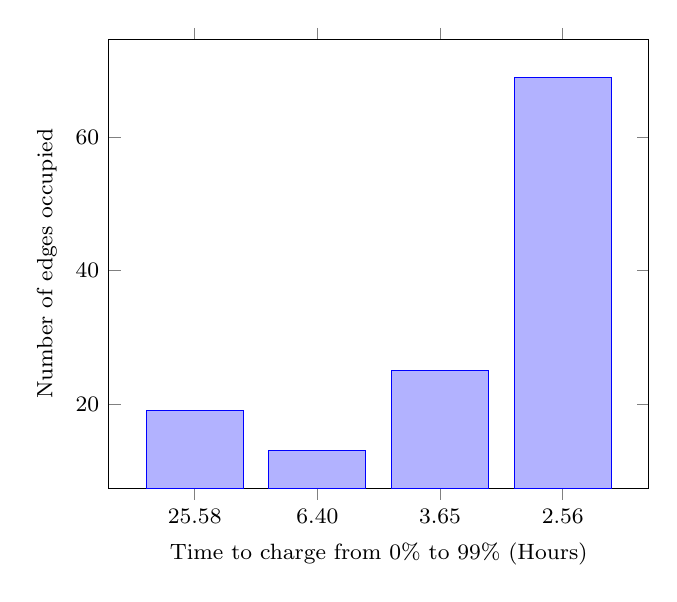
\begin{tikzpicture}
		\begin{axis}[ybar, xmin=0.3, xmax=4.7, font=\footnotesize, xtick={1,2,3,4},xticklabels={25.58, 6.40, 3.65, 2.56},
			ylabel=Number of edges occupied, bar width=35pt, xlabel=Time to charge from 0\% to 99\% (Hours)]
			\addplot coordinates{(1,19) (2,13) (3,25) (4,69)};
		\end{axis}
	\end{tikzpicture}
	\caption{Histogram of charge rates, where each rate is described by how must time it would take to charge a bus from 0\% to 99\%.}
	\label{fig:chargeRateHistogram}
\end{figure}













